\graphicspath{ {imgs/} }
\documentclass[main.tex]{subfiles}
\begin{document}
\chapter{Current Approaches}\label{chap:approaches}
This chapter illustrates the current state of the art in the field of automated nodule detection. Roughly the field can be divided among the used methods in the \emph{classical} approaches and the deep learning approaches. It also describes how this thesis is situated in the field and what is done differently compared to previous papers.

\section{Classical Approaches}
Nodule detection is a complex and potentially life-saving task, so it makes sense that there is a scientific community dedicated to finding algorithmic approaches to aid the radiologists. In this section, some of the published papers in this domain and the techniques they use will be explained. In principal algorithms applied to the lung CT images can be subdivided into several stages (as can be for example seen in~\ref{fig:pipeline}). Similar to other computer vision algorithms those can be roughly clustered in the following: Segmentation, Candidate Selection, Classification.


\begin{figure}[ht]
\centering
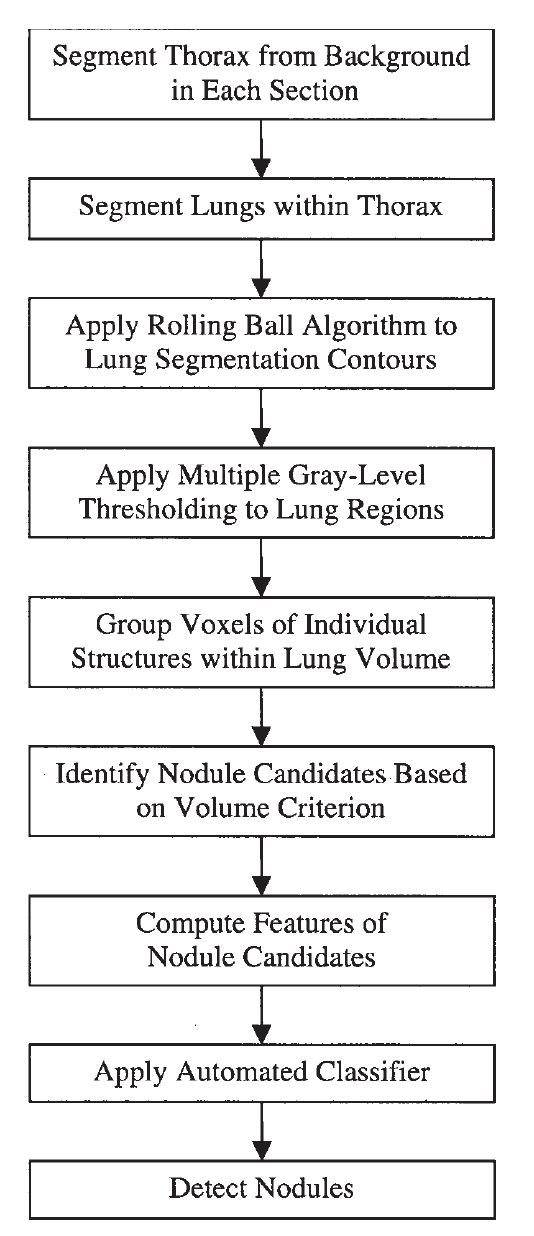
\includegraphics[scale=0.5]{armato_pipeline.png}
\caption{This image is taken from Armato's paper ``Computerized Detection
of Pulmonary Nodules on CT Scans''~\cite{armato1999computerized} and describes on one specific example how a traditional approach towards nodule detection is modeled.}
\label{fig:pipeline}
\end{figure}


\subsection{Segmentation}
A lung CT scan contains more anatomical structure than just the lung area. It is necessary to exclude the trachea, heart as well as the spine from the slices in order to solely focus on the lung tissue. Armato et al.~\cite{armato1999computerized,armato2001automated} use for example twice a gray-value thresholding. First with a fixed parameter to exclude the background (the air surrounding the patient) and a second time with a varying threshold based on the distribution of gray values in the slice. Roughly two peaks mark the heart and the more solid surrounding tissue (which result in brighter values on the scan image) and a lower peak for the darker region - the threshold is then chosen between the two peaks. Gurcan et al.~\cite{gurcan2002lung} use k-means clustering (with $k=2$) on the histogram to separate the two groups. 

Juxtapleural nodules can pose a problem in this scenario since they lie closely connected to the membrane (pleura) that lines the lung and might be erroneously excluded. They produce cavities on the initially segmented lung and need to be corrected. A rolling ball filter can be used to smooth the contoures of the lung again and rightly add the juxtapleural nodules to the inner lung region~\cite{armato1999computerized}. Another approach, used by Gurcan et al.~\cite{gurcan2002lung} is comparing the distance between two points measured along the contour that was formed by the initial segmentation and comparing it to the Euclidean distance between the points. If the ratio is bigger than a preselected threshold the points are again connected with a line. The final segmentation looks similar to Figure~\ref{fig:segmentation}.

\begin{figure}[ht]
\centering
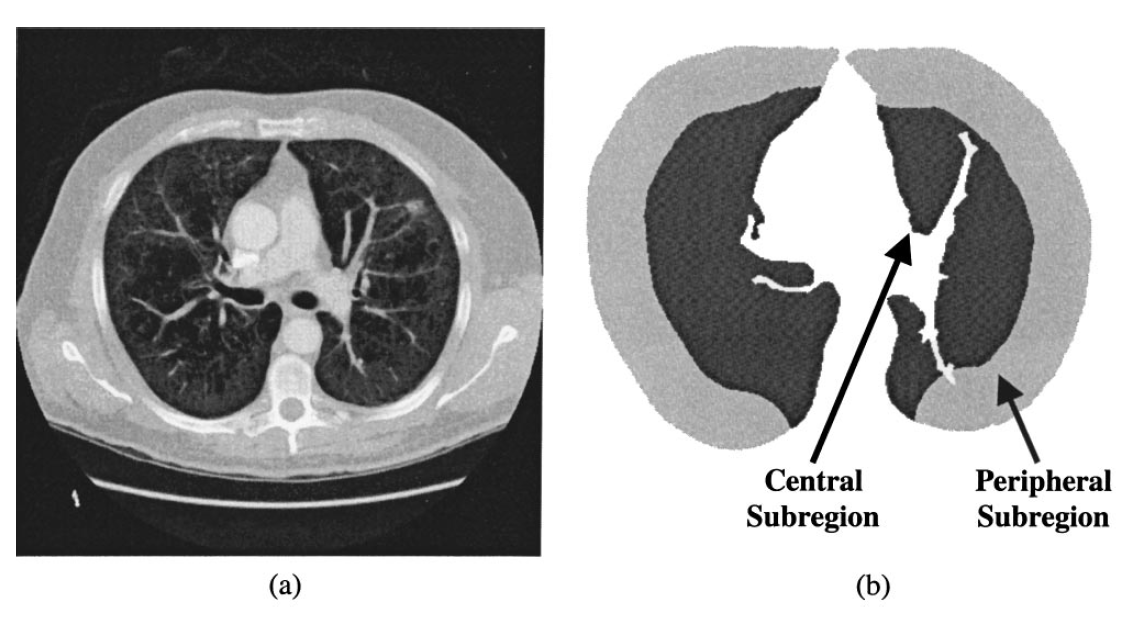
\includegraphics[scale=0.7]{gurcan_lungsegmentations.png}
\caption{This image is taken from Gurcan's paper ``Lung nodule detection on thoracic computed tomography images: Preliminary evaluation of a computer-aided diagnosis system''~\cite{gurcan2002lung} and shows the result of the segmentation process.}
\label{fig:segmentation}
\end{figure}


\subsection{Candidate Selection}
From the segmented lung region nodule candidates are selected. This selection can be done either by intensity- or model-based methods. The following text describes exemplary one method for each of the two types of algorithms and highlights concerns or limits of those. Armato et al.~\cite{armato1999computerized} use a multiple thresholding of the slices to obtain a set of $15$ CT scans that only contain pixels above an increasing threshold. Now the 10 neighborhood of all on-pixels is used to group pixels together in structures, which are then classified by their volume. All structures that have a volume less than $14.1cm^3$ are nodule candidates and the others are disregarded.

Another approach involves using a predefined geometrical model to find the nodule candidates. Ye et al.~\cite{ye2009shape} use, for example, a shape index as defined in Equation~\ref{eq:SI} (this index is basically just a rescaled version of the original shape index that produces values between $-1,1$ to $0,1$) to classify candidates based on the shape of their surface. $k(p)$ are the values of the principal curvature in a point of interest $p$. Nodules obtain a higher score (closer to $1$) compared to blood vessels, which have a prolonged shape. 

\begin{equation} \label{eq:SI}
SI(p)=\frac{1}{2}-\frac{1}{\pi}arctan\frac{k_1(p)+k_2(p)}{k_1(p)-k_2(p)}
\end{equation}

Using sphericity as a strong nodule indicator may lead to a model that is highly sensitive to only one type of nodules while ignoring nodules that lie close to the chest wall and are not perfectly round or GGO nodules that are more diffuse in their morphology. Model-based algorithms, on the other hand, have the advantage of being able to incorporate a priori knowledge more easily. Different model parameters, for example, can be fine-tuned due to the vessel density in a region of the lung - e.g. blood vessels are more common in the central region of the lung. The extracted nodule candidates can now be further processed in the classification step.


\subsection{Classification}
The candidates have to be classified to separate nodules between cancerous and non-malicious types. The classification itself can again be split into several steps, but this section will only highlight a few examples to give an overview. Armato et~al.~\cite{armato1999computerized} and Gurcan et~al.~\cite{gurcan2002lung} use a linear discriminant analysis classifier along several nodule features like volume, sphericity, the radius of an equivalent sphere and more to separate real nodules from other structures which have been found by the before described selection process. Firmino et~al.~\cite{firmino2014computer} provide a very rich comparison of different CAD methods and their performance, which can be seen in Figure~\ref{fig:firmino_comp}.

\begin{figure}[ht]
\centering
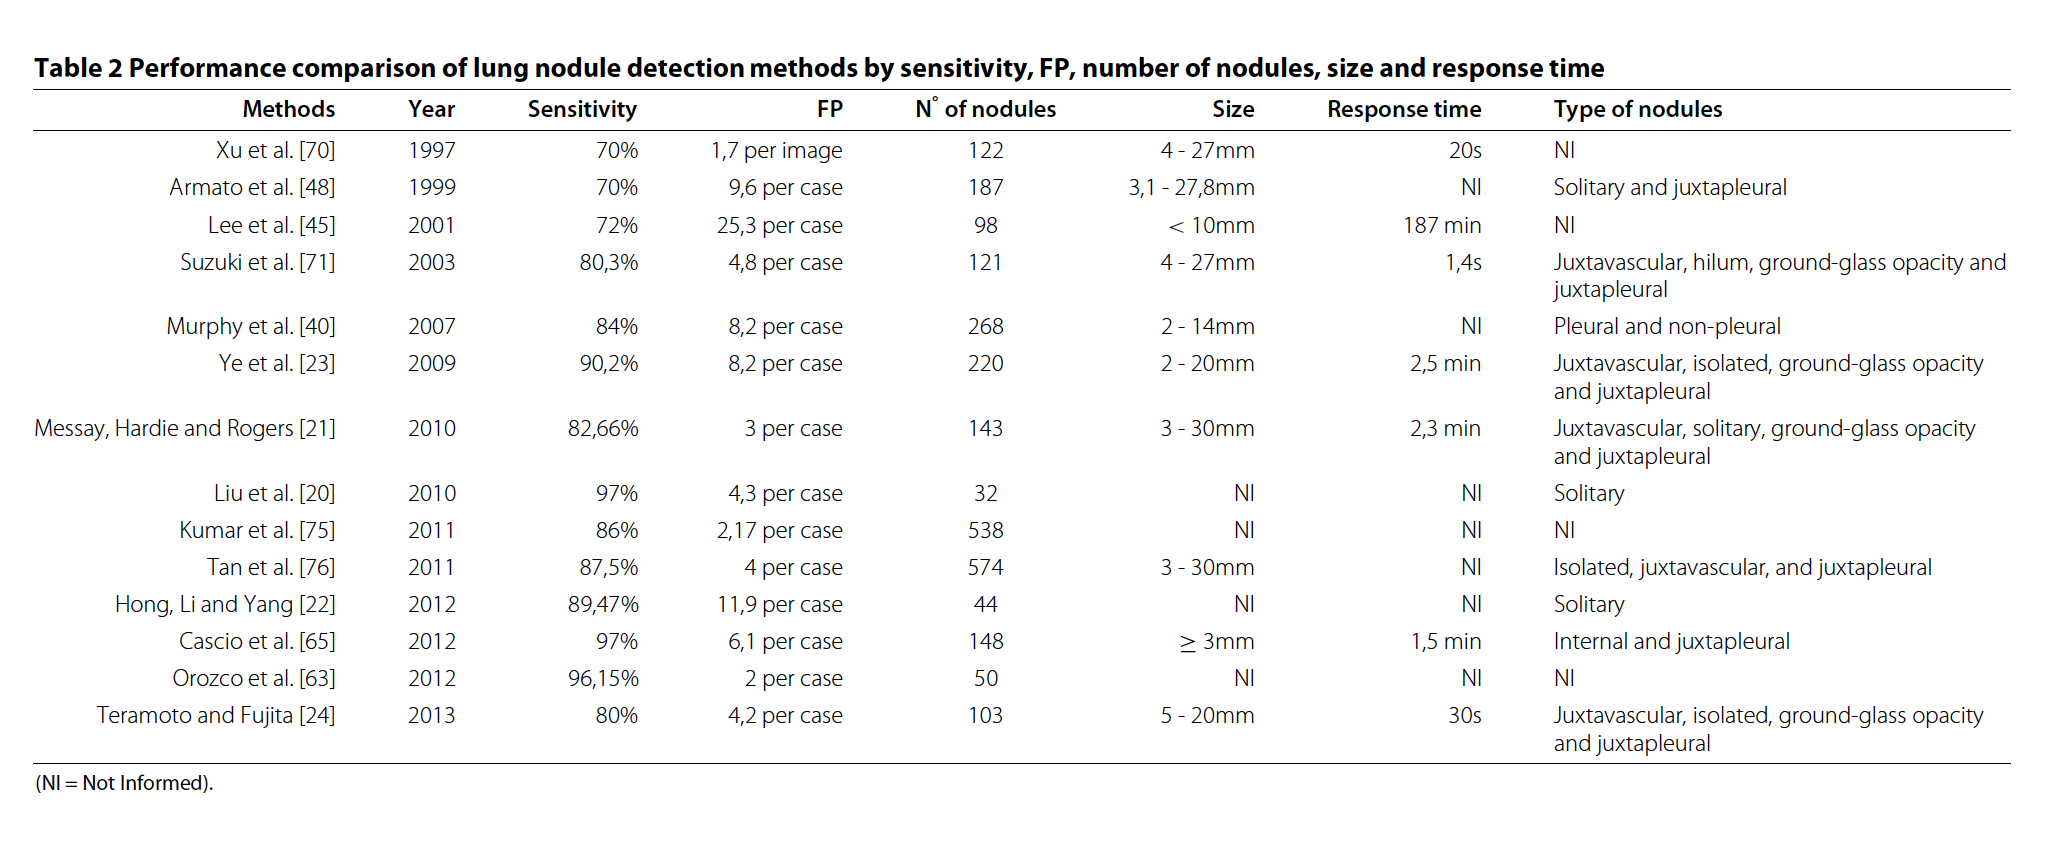
\includegraphics[width=\textwidth]{firmino_comparison.png}
\caption{This table is taken from Firmino et~al.'s paper ``Computer-aided detection system for lung cancer in computed tomography scans: Review and future prospects''~\cite{firmino2014computer} and shows the performance of different algorithms. It is noticable how the number nodules used for training differ widely between the cases.}
\label{fig:firmino_comp}
\end{figure}


\section{Deep Learning Approaches}
A deep learning approach as defined in this thesis is any approach that utilizes in at least one of the above-explained steps a neural network with more than $2$ layers. All of the found papers use a mixed strategy: using more classical candidate selection strategies and using the neural network only in the final classification step. From those papers only two other papers use 3D Convolutional Neural Networks: Anirudh et al.~\cite{anirudh2016lung} and Huang et al.~\cite{huang2017lung}. The first one uses point estimates in the CT scan that have to be manually provided (by the radiologists for example). Those points are used as the seed point in a region growing method and the resulting 3-dimensional structure is fed into a convolutional network to determine whether it is a nodule or not. This means that by principal it is not possible to detect nodules that the radiologist missed. Huang's approach utilizes classic computer vision algorithms (a curvature based method and Bayesian filters) to find candidate areas in the scan. The resulting cubes are aligned to their principal direction which normalizes the nodule representation. A 3D convolutional network is then used for classification. The drawback with this method is that GGO nodules and juxtapleural nodules are excluded because the candidate selection process does not support them.


\section{This Thesis}
Where can this thesis be positioned in the field of Lung CT analysis and nodule detection? Given the sections above it is clear that it is part of the deep learning approaches, but differs in the sense that no prior candidate selection is performed on the data. The classification is based on raw CT scan patches that are fed to the network as is. The amount of data used for the training process also differs compared to the more classical papers. $2565$ nodule and healthy patches have been used for the classification, which is way more than commonly found in the literature. This thesis is also concerned with pure nodule detection and no further rating of the found structures, like for example their malignancy. This means that no further features of the nodule have been used for the training process.



\end{document}
